\section{HHL Algorithmus}

\subsubsection{Übersicht}

    \begin{frame}
    \frametitle{Übersicht}
        Vergleich klassische zur quanten Version

        \hfil
        \begin{columns}[c]
            \begin{column}{0.6\hsize}\centering
            Klassisch
            $$A \vec{x} = \vec{b}$$
            $$\vec{x} = A^{-1}\vec{b}$$
            \end{column}

            \begin{column}{0.4\hsize}
            Quanten Version
            $$A \ket{x} = \ket{b}$$
            $$\ket{x} = A^{-1}\ket{b}$$
            \end{column}
        \end{columns}

    

    \end{frame}


    \begin{frame}
    \frametitle{Übersicht}

        \hfil

        $A$ kann man auch in der Spektralzerlegung darstellen

        \hfil
        \begin{columns}[c]
            \begin{column}{0.4\hsize}\centering
            $$A = \sum_{i=0}^{2^{n_b}-1} \lambda_i \ket{u_i}\bra{u_i}$$
            $$A^{-1} = \sum_{i=0}^{2^{n_b}-1} \lambda_i^{-1} \ket{u_i}\bra{u_i}$$
            \end{column}

            \begin{column}{0.6\hsize}
            \begin{itemize}
            \item   $\lambda_i$ sind Eigenwerte von A
            \item   $\ket{u_i}$ sind Eigenvektoren von A
            \end{itemize}
 
            \end{column}
        \end{columns}

        \hfil

        \hfil

        $\vec{b}$ kann in der Eigenbasis von $A$ dargestellt werden 

        \hfil

        \begin{columns}[c]
            \begin{column}{0.4\hsize}\centering
            $$\ket{b} = \sum_{j=0}^{2^{n_b}-1} b_j\ket{u_j}$$
            \end{column}
            \begin{column}{0.6\hsize}
            \begin{itemize}
            \item   $b_i$ sind die koeffizienten von $\vec{b}$
            \item   $\ket{u_i}$ sind Eigenvektoren von A
            \end{itemize}
 
            \end{column}
        \end{columns}



   \end{frame}

    \begin{frame}
    \frametitle{Übersicht}

        Setzen wir nun alles ein:

        \hfil
        $$\ket{x} = A^{-1} \ket{b} = \left( \sum_{i=0}^{2^{n_b}-1} \lambda_i^{-1} \ket{u_i}\bra{u_i} \right) \left( \sum_{j=0}^{2^{n_b}-1} b_j\ket{u_j} \right)$$
        $$\ket{x}= \sum_{i=0}^{2^{n_b}-1} \sum_{j=0}^{2^{n_b}-1} \lambda_i^{-1} \ket{u_i}\bra{u_i} b_j\ket{u_j}$$
        $$\ket{x}= \sum_{i=0}^{2^{n_b}-1} \sum_{j=0}^{2^{n_b}-1} \lambda_i^{-1} b_j\ket{u_i}\braket{u_i| u_j}$$
        $$\ket{x} = \sum_{i=0}^{2^{n_b}-1} \sum_{j=0}^{2^{n_b}-1} \lambda_i^{-1} b_j\ket{u_i}\delta_{ij}$$

    \end{frame}


    \begin{frame}
    \frametitle{Übersicht}
        Setzen wir nun alles ein (Fort.):

        \hfil
        $$\ket{x} = \sum_{i=0}^{2^{n_b}-1} \sum_{j=0}^{2^{n_b}-1} \lambda_i^{-1} b_j\ket{u_i}\delta_{ij}$$
        $$\ket{x} =  A^{-1} \ket{b} = \sum_{i=0}^{2^{n_b}-1} \lambda_i^{-1} b_j\ket{u_j}$$
        $$\ket{x} =  A^{-1} \ket{b} = \sum_{i=0}^{2^{n_b}-1} \lambda_i^{-1} b_j\ket{u_j}$$

    \end{frame}

    \begin{frame}
    \frametitle{Übersicht}
        \begin{enumerate}
            \item Ermittle die Eigenwerte und Eigenvektoren von $A$
            \item bilde $\ket{b}$ in Eigenbasis $A$ ab
            \item  Invertiert Eigenwerte
            \item lies das Ergebnis $\ket{x}$ aus
        \end{enumerate}
    \end{frame}

\subsubsection{Der Algorithmus}

    \begin{frame}
    \frametitle{Der Algorithmus}

        \textbf{Ablauf}
        \begin{enumerate}
            \item State Preparation
            \begin{itemize}
                \item Enkodiere Vektor und Matrix in Quanten Computer
            \end{itemize}
            \item Quantum Phase Estimation
            \begin{itemize}
                \item ermittle Eigenwerte und Eigenvektoren 
                \item bilde $\ket{b}$ in Eigenbasis $A$ ab
            \end{itemize}
            \item Ancilla Bit Rotation 
            \begin{itemize}
                \item  Invertiert Eigenwerte
            \end{itemize}
            \item Inverse Quantum Phase Estimation
             \begin{itemize}
                \item löst verschränkte Qubits auf
            \end{itemize}
            
            \item Messung
             \begin{itemize}
                \item liest das Ergebnis $\ket{x}$ aus
            \end{itemize}
 
        \end{enumerate}

    \end{frame}

    \begin{frame}
    \frametitle{Quantum Circuit}
    \begin{center}
    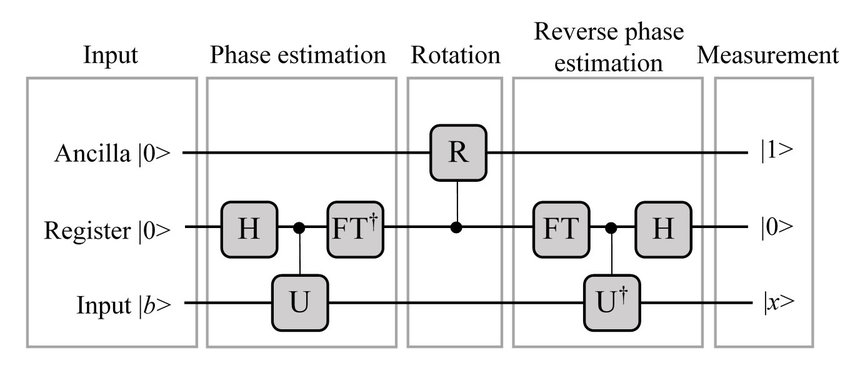
\includegraphics[width=10cm]{img/hhl_circuit.jpg}
    \end{center}

    \begin{enumerate}
        \item Ancilla (Helfer): a-register
        \begin{itemize}
            \item Indikator qubit - zeigt an ob Zustände verschränkt sind
        \end{itemize}

        \item Register: c-register
        \begin{itemize}
            \item beinhaltet später die eigenwerte
        \end{itemize}
        
        \item Input: b-register 
        \begin{itemize}
            \item beinhaltet den Vektor $\vec{b}$
        \end{itemize}
        
    \end{enumerate}
   \end{frame}

\begin{frame}
    \frametitle{Quantum Circuit}
    \hfil

    Wo befindet sich die Matrix $A$?
    \begin{center}
    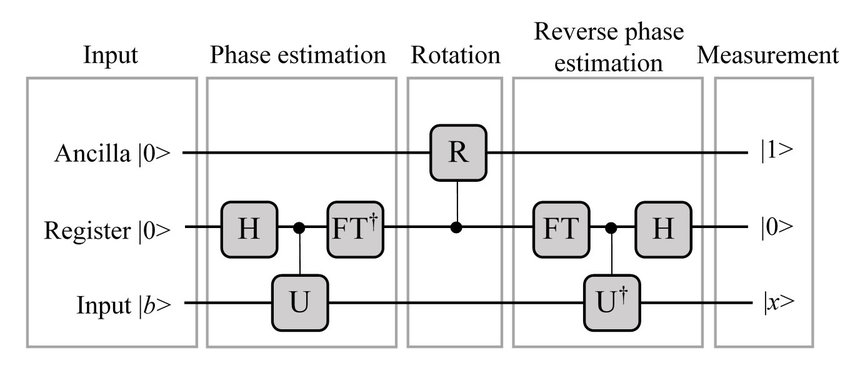
\includegraphics[width=10cm]{img/hhl_circuit.jpg}
    \end{center}

    \hfil
    Wir als Unitary (Einheitsmatrix) in die Phase Estimation enkodiert.
    $$U = e^{iAt}$$
   \end{frame}

\begin{frame}
    \frametitle{State }
    \hfil

    Wo befindet sich die Matrix $A$?
    \begin{center}
    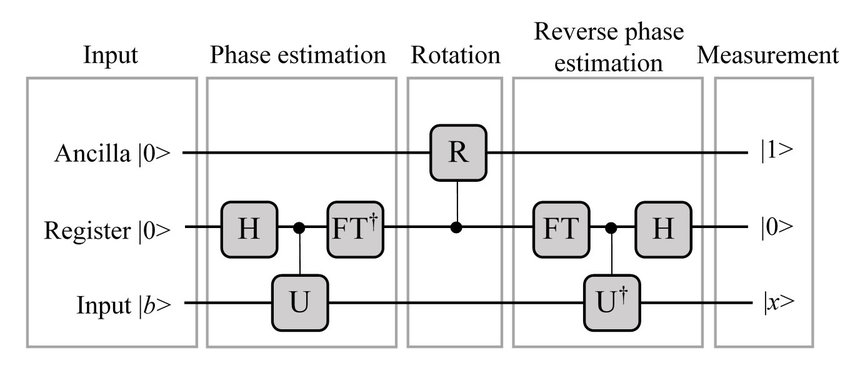
\includegraphics[width=10cm]{img/hhl_circuit.jpg}
    \end{center}

    \hfil
    Wir als Unitary (Einheitsmatrix) in die Phase Estimation enkodiert.
    $$U = e^{iAt}$$
\end{frame}


